% Experiment: calibration under the null and localisation after calibration.
% Tables are rendered from the study artifact by
%   python paper/scripts/render_calibrated_tables.py \
%       --summary artifacts/runs/calibrated-study-v3/summary.json \
%       --out-prefix paper/sections/calibrated

\subsection{Experiment 2: Calibration Under the Null}
\label{sec:calibration}

The decomposed pathway of Section~\ref{sec:method} calibrates each family with an
asymptotic null. Two of its assumptions are testable in isolation: that the rank
transform makes the correlation difference pivotal, and that Bonferroni over dependent
edges is a usable level control. This experiment measures both, and it separates the
\emph{decision} (is there drift, and in which family?) from the \emph{ordering} (which
features carry it).

\paragraph{Protocol}
Null populations receive no injection, so a family-wise rejection is a false alarm; this
isolates calibration from power. Localisation conditions inject a known change and score
Recall@3 against the frozen truth, with the uniform-random Recall@3 chance line
$3/d = 15.0\%$ as reference.
Every method in a cell is evaluated on the identical reference/current pair, so
comparisons are paired by construction and tested with Holm-corrected paired tests.
Each configuration is re-run under the permutation path (peeling, max-edge aggregation,
unsplit $\alpha$, rank-transform statistic) and under the asymptotic path (published
decomposed, threshold-split decomposed, KS-only, copula-only, KS with raw Pearson). The
synthetic null populations are a Gaussian pool, a zero-inflated pool with mass at zero and
deliberate ties, and a multivariate Student-$t$ pool ($\nu = 3$) with heavy tails; the
real pools are CICIDS2017 Tuesday (validation) and Wednesday--Friday (held-out) windows
drawn from the prepared splits. Real-data trials resample a fixed set of disjoint
$800$-row blocks, so the block-clustered interval, not the binomial one, is the interval
to quote for those rows. The calibration and localisation tables are generated by
\path{paper/scripts/render_calibrated_tables.py} from
\path{artifacts/runs/calibrated-study-v3/summary.json} and the exchangeability table by
\path{paper/scripts/render_blocknull_table.py} from
\path{artifacts/runs/calibrated-blocknull-v2/summary.json}; the only transcribed table
is the NSL-KDD null table, whose counts come from
\path{artifacts/runs/real-null-v1}.

\begin{table*}[!tp]
\centering
\caption{Family-wise false-alarm rate with nothing injected (nominal 5\%, 199 permutations, 500 trials per cell; column keys: \textup{\textit{Dec.}}\ = decomposed Copula--KS as published, \textup{\textit{Dec.\ ($\alpha$/2)}} = the same with the $\alpha$ split, \textup{\textit{KS}} and \textup{\textit{Cop.}}\ = single pathways, \textup{\textit{Pear.}}\ = raw Pearson, \textup{\textit{Cal.\ max-edge}} and \textup{\textit{Cal.\ peel}} = the calibrated policy with the max-edge and greedy-peeling orders, \textup{\textit{Peel, no split}} and \textup{\textit{Peel, rank}} = peeling with an unsplit $\alpha$ and with the rank copula statistic; entries are point estimates; 95\% Wilson intervals are in \textup{\texttt{summary.json}} and in the repository's markdown rendering). Real-data rows draw both windows from one row-disjoint block of a single split, so they are null pairs that resample a fixed block set; the block-clustered interval in the artifact is the one to quote there.}
\label{tab:null-calibration}
\small
\resizebox{\textwidth}{!}{%
\begin{tabular}{lrrrrrrrrr}
\toprule
Null population & Dec.\ & Dec.\ ($\alpha$/2) & KS & Cop.\ & Pear.\ & Cal.\ max-edge & Cal.\ peel & Peel, no split & Peel, rank \\
\midrule
Gaussian & 8.6 & 3.8 & 3.8 & 4.8 & 4.4 & 3.8 & 3.8 & 9.8 & 3.4 \\
Zero-inflated, tied & 9.8 & 7.4 & 0.2 & 9.6 & 100.0 & 5.8 & 5.8 & 10.6 & 5.2 \\
Multivariate $t_3$ & 45.8 & 36.2 & 2.6 & 44.8 & 100.0 & 3.2 & 3.2 & 8.4 & 3.4 \\
CICIDS2017 Tuesday (no injection) & 59.0 & 54.4 & 2.0 & 59.0 & 100.0 & 4.4 & 4.4 & 10.2 & 3.8 \\
CICIDS2017 held-out (no injection) & 57.8 & 53.2 & 1.2 & 57.8 & 99.8 & 3.2 & 3.2 & 8.6 & 3.2 \\
\bottomrule
\end{tabular}
}
\end{table*}

\begin{table*}[!tp]
\centering
\caption{Recall@3 (\%) per condition against the uniform-random line $3/d = 15.0$\% (every condition injects the same number of truth features per window, including the permutation, whose truth spans two windows). Peeling is the calibrated ranking; its decision rule is the joint family-wise test of Table~\ref{tab:null-calibration}.}
\label{tab:localization}
\footnotesize
\renewcommand{\arraystretch}{0.90}
\resizebox{\textwidth}{!}{%
\begin{tabular}{llrrrrrrrr}
\toprule
Dataset & Condition & Chance & Decomposed & KS & Copula & Pearson & Max-edge & Peeling & Peeling (rank) \\
\midrule
gaussian & mean\_0.2\_k2 & 15.0 & 55.0 & 72.5 & 22.5 & 25.0 & 67.5 & 67.5 & 67.5 \\
gaussian & mean\_0.5\_k2 & 15.0 & 100.0 & 100.0 & 22.5 & 25.0 & 100.0 & 100.0 & 100.0 \\
gaussian & mean\_0.5\_k2\_sparse20 & 15.0 & 32.5 & 27.5 & 30.0 & 22.5 & 30.0 & 30.0 & 35.0 \\
gaussian & mean\_0.5\_k2\_sparse5 & 15.0 & 25.0 & 15.0 & 25.0 & 22.5 & 20.0 & 20.0 & 22.5 \\
gaussian & paircorr\_0.3\_k2 & 15.0 & 70.0 & 17.5 & 70.0 & 70.0 & 67.5 & 67.5 & 60.0 \\
gaussian & paircorr\_0.8\_k2 & 15.0 & 100.0 & 17.5 & 100.0 & 100.0 & 100.0 & 100.0 & 100.0 \\
gaussian & permute\_k1 & 15.0 & 100.0 & 10.0 & 100.0 & 100.0 & 100.0 & 100.0 & 100.0 \\
gaussian & permute\_k2 & 15.0 & 62.5 & 17.5 & 62.5 & 52.5 & 55.0 & 95.0 & 87.5 \\
gaussian & permute\_k2\_sparse20 & 15.0 & 37.5 & 17.5 & 47.5 & 37.5 & 37.5 & 37.5 & 37.5 \\
gaussian & permute\_k5 & 15.0 & 32.0 & 11.0 & 32.0 & 26.0 & 24.0 & 59.0 & 57.0 \\
gaussian & scale\_0.5\_k2 & 15.0 & 100.0 & 100.0 & 22.5 & 25.0 & 100.0 & 100.0 & 100.0 \\
gaussian & scale\_0.5\_k2\_sparse20 & 15.0 & 30.0 & 27.5 & 22.5 & 22.5 & 35.0 & 35.0 & 30.0 \\
gaussian & scale\_2\_k2 & 15.0 & 100.0 & 100.0 & 22.5 & 25.0 & 100.0 & 100.0 & 100.0 \\
\midrule
multivariate\_t3 & mean\_0.2\_k2 & 15.0 & 40.0 & 70.0 & 10.0 & 7.5 & 55.0 & 55.0 & 60.0 \\
multivariate\_t3 & mean\_0.5\_k2 & 15.0 & 92.5 & 100.0 & 10.0 & 7.5 & 100.0 & 100.0 & 100.0 \\
multivariate\_t3 & mean\_0.5\_k2\_sparse20 & 15.0 & 15.0 & 32.5 & 12.5 & 7.5 & 20.0 & 20.0 & 22.5 \\
multivariate\_t3 & mean\_0.5\_k2\_sparse5 & 15.0 & 15.0 & 7.5 & 15.0 & 7.5 & 7.5 & 7.5 & 17.5 \\
multivariate\_t3 & paircorr\_0.3\_k2 & 15.0 & 60.0 & 7.5 & 60.0 & 37.5 & 60.0 & 60.0 & 60.0 \\
multivariate\_t3 & paircorr\_0.8\_k2 & 15.0 & 100.0 & 7.5 & 100.0 & 77.5 & 100.0 & 100.0 & 100.0 \\
multivariate\_t3 & permute\_k1 & 15.0 & 100.0 & 0.0 & 100.0 & 65.0 & 100.0 & 100.0 & 100.0 \\
multivariate\_t3 & permute\_k2 & 15.0 & 70.0 & 7.5 & 70.0 & 45.0 & 65.0 & 92.5 & 92.5 \\
multivariate\_t3 & permute\_k2\_sparse20 & 15.0 & 40.0 & 7.5 & 42.5 & 15.0 & 30.0 & 30.0 & 32.5 \\
multivariate\_t3 & permute\_k5 & 15.0 & 36.0 & 18.0 & 36.0 & 32.0 & 32.0 & 58.0 & 59.0 \\
multivariate\_t3 & scale\_0.5\_k2 & 15.0 & 100.0 & 100.0 & 10.0 & 7.5 & 100.0 & 100.0 & 100.0 \\
multivariate\_t3 & scale\_0.5\_k2\_sparse20 & 15.0 & 12.5 & 25.0 & 12.5 & 7.5 & 20.0 & 20.0 & 17.5 \\
multivariate\_t3 & scale\_2\_k2 & 15.0 & 97.5 & 100.0 & 10.0 & 7.5 & 97.5 & 97.5 & 100.0 \\
\midrule
real\_heldout & mean\_0.2\_k2 & 15.0 & 100.0 & 100.0 & 15.0 & 12.5 & 100.0 & 100.0 & 100.0 \\
real\_heldout & mean\_0.5\_k2 & 15.0 & 100.0 & 100.0 & 15.0 & 12.5 & 100.0 & 100.0 & 100.0 \\
real\_heldout & mean\_0.5\_k2\_sparse20 & 15.0 & 57.5 & 100.0 & 57.5 & 15.0 & 92.5 & 95.0 & 87.5 \\
real\_heldout & mean\_0.5\_k2\_sparse5 & 15.0 & 40.0 & 32.5 & 42.5 & 15.0 & 35.0 & 35.0 & 47.5 \\
real\_heldout & paircorr\_0.3\_k2 & 15.0 & 55.0 & 15.0 & 55.0 & 30.0 & 55.0 & 55.0 & 57.5 \\
real\_heldout & paircorr\_0.8\_k2 & 15.0 & 60.0 & 15.0 & 60.0 & 25.0 & 60.0 & 60.0 & 60.0 \\
real\_heldout & permute\_k1 & 15.0 & 100.0 & 5.0 & 100.0 & 60.0 & 100.0 & 100.0 & 100.0 \\
real\_heldout & permute\_k2 & 15.0 & 65.0 & 15.0 & 65.0 & 37.5 & 57.5 & 95.0 & 97.5 \\
real\_heldout & permute\_k2\_sparse20 & 15.0 & 62.5 & 15.0 & 62.5 & 22.5 & 57.5 & 60.0 & 62.5 \\
real\_heldout & permute\_k5 & 15.0 & 31.0 & 16.0 & 31.0 & 26.0 & 29.0 & 60.0 & 60.0 \\
real\_heldout & scale\_0.5\_k2 & 15.0 & 100.0 & 100.0 & 15.0 & 12.5 & 100.0 & 100.0 & 100.0 \\
real\_heldout & scale\_0.5\_k2\_sparse20 & 15.0 & 60.0 & 97.5 & 55.0 & 20.0 & 85.0 & 85.0 & 85.0 \\
real\_heldout & scale\_2\_k2 & 15.0 & 100.0 & 100.0 & 15.0 & 12.5 & 100.0 & 100.0 & 100.0 \\
\midrule
real\_tuesday & mean\_0.2\_k2 & 15.0 & 100.0 & 100.0 & 17.5 & 10.0 & 100.0 & 100.0 & 100.0 \\
real\_tuesday & mean\_0.5\_k2 & 15.0 & 100.0 & 100.0 & 17.5 & 10.0 & 100.0 & 100.0 & 100.0 \\
real\_tuesday & mean\_0.5\_k2\_sparse20 & 15.0 & 60.0 & 100.0 & 55.0 & 20.0 & 95.0 & 95.0 & 95.0 \\
real\_tuesday & mean\_0.5\_k2\_sparse5 & 15.0 & 42.5 & 55.0 & 40.0 & 15.0 & 57.5 & 57.5 & 60.0 \\
real\_tuesday & paircorr\_0.3\_k2 & 15.0 & 55.0 & 27.5 & 55.0 & 32.5 & 55.0 & 55.0 & 57.5 \\
real\_tuesday & paircorr\_0.8\_k2 & 15.0 & 65.0 & 27.5 & 65.0 & 30.0 & 65.0 & 65.0 & 62.5 \\
real\_tuesday & permute\_k1 & 15.0 & 100.0 & 20.0 & 100.0 & 55.0 & 100.0 & 100.0 & 100.0 \\
real\_tuesday & permute\_k2 & 15.0 & 65.0 & 27.5 & 65.0 & 40.0 & 57.5 & 95.0 & 92.5 \\
real\_tuesday & permute\_k2\_sparse20 & 15.0 & 60.0 & 27.5 & 60.0 & 22.5 & 50.0 & 52.5 & 60.0 \\
real\_tuesday & permute\_k5 & 15.0 & 34.0 & 19.0 & 34.0 & 24.0 & 29.0 & 58.0 & 60.0 \\
real\_tuesday & scale\_0.5\_k2 & 15.0 & 100.0 & 100.0 & 17.5 & 10.0 & 100.0 & 100.0 & 100.0 \\
real\_tuesday & scale\_0.5\_k2\_sparse20 & 15.0 & 67.5 & 100.0 & 55.0 & 15.0 & 90.0 & 90.0 & 90.0 \\
real\_tuesday & scale\_2\_k2 & 15.0 & 100.0 & 100.0 & 17.5 & 10.0 & 100.0 & 100.0 & 100.0 \\
\midrule
zero\_inflated\_tied & mean\_0.2\_k2 & 15.0 & 100.0 & 100.0 & 12.5 & 12.5 & 100.0 & 100.0 & 100.0 \\
zero\_inflated\_tied & mean\_0.5\_k2 & 15.0 & 100.0 & 100.0 & 12.5 & 12.5 & 100.0 & 100.0 & 100.0 \\
zero\_inflated\_tied & mean\_0.5\_k2\_sparse20 & 15.0 & 100.0 & 100.0 & 75.0 & 12.5 & 100.0 & 100.0 & 100.0 \\
zero\_inflated\_tied & mean\_0.5\_k2\_sparse5 & 15.0 & 17.5 & 47.5 & 17.5 & 12.5 & 32.5 & 32.5 & 35.0 \\
zero\_inflated\_tied & paircorr\_0.3\_k2 & 15.0 & 72.5 & 20.0 & 75.0 & 20.0 & 67.5 & 67.5 & 60.0 \\
zero\_inflated\_tied & paircorr\_0.8\_k2 & 15.0 & 100.0 & 20.0 & 100.0 & 45.0 & 100.0 & 100.0 & 100.0 \\
zero\_inflated\_tied & permute\_k1 & 15.0 & 25.0 & 25.0 & 25.0 & 20.0 & 30.0 & 30.0 & 5.0 \\
zero\_inflated\_tied & permute\_k2 & 15.0 & 40.0 & 20.0 & 40.0 & 25.0 & 32.5 & 32.5 & 22.5 \\
zero\_inflated\_tied & permute\_k2\_sparse20 & 15.0 & 12.5 & 20.0 & 15.0 & 15.0 & 10.0 & 10.0 & 12.5 \\
zero\_inflated\_tied & permute\_k5 & 15.0 & 26.0 & 20.0 & 25.0 & 21.0 & 24.0 & 24.0 & 17.0 \\
zero\_inflated\_tied & scale\_0.5\_k2 & 15.0 & 100.0 & 100.0 & 12.5 & 12.5 & 100.0 & 100.0 & 100.0 \\
zero\_inflated\_tied & scale\_0.5\_k2\_sparse20 & 15.0 & 97.5 & 100.0 & 22.5 & 15.0 & 97.5 & 97.5 & 97.5 \\
zero\_inflated\_tied & scale\_2\_k2 & 15.0 & 100.0 & 100.0 & 12.5 & 12.5 & 100.0 & 100.0 & 100.0 \\
\bottomrule
\end{tabular}
}
\end{table*}

\begin{table*}[!tp]
\centering
\caption{Paired Recall@3 differences in percentage points (peeling minus baseline) on the same 20 seeds, one row per condition--population cell; $^{*}$ marks Holm-adjusted $p < 0.05$ within each cell across the 9 baselines (Wilcoxon signed-rank, or a sign test when $n < 10$). Positive is better for peeling. Cop = copula asymptotic, Dec = decomposed asymptotic, Bonf = decomposed ($\alpha/2$), KS = marginal KS pathway, KS$+$Pear = KS plus raw Pearson, Pear = raw Pearson relational, Max = calibrated max-edge without peeling, Sep$_\alpha$ = peeling without $\alpha$ split, Rank = peeling on rank-copula statistic. Win/loss/tie counts and raw $p$-values are in \textup{\texttt{summary.json}}.}
\label{tab:paired-tests}
\scriptsize
\renewcommand{\arraystretch}{0.86}
\begin{tabular*}{\textwidth}{@{\extracolsep{\fill}}lrrrrrrrrr}
\toprule
Cell & \multicolumn{9}{c}{$\Delta$ Recall@3 vs each baseline} \\
 & Cop & Dec & Bonf & KS & KS$+$Pear & Pear & Max & Sep$_\alpha$ & Rank \\
\midrule
\texttt{gaussian}:mean\_0.2\_k2 & $+$45.0$^{*}$ & $+$12.5 & $+$12.5 & $-$5.0 & $+$10.0 & $+$42.5$^{*}$ & 0.0 & 0.0 & 0.0 \\
\texttt{gaussian}:mean\_0.5\_k2 & $+$77.5$^{*}$ & 0.0 & 0.0 & 0.0 & 0.0 & $+$75.0$^{*}$ & 0.0 & 0.0 & 0.0 \\
\texttt{gaussian}:mean\_0.5\_k2\_sparse20 & 0.0 & $-$2.5 & $-$2.5 & $+$2.5 & $+$7.5 & $+$7.5 & 0.0 & 0.0 & $-$5.0 \\
\texttt{gaussian}:mean\_0.5\_k2\_sparse5 & $-$5.0 & $-$5.0 & $-$5.0 & $+$5.0 & $-$2.5 & $-$2.5 & 0.0 & 0.0 & $-$2.5 \\
\texttt{gaussian}:paircorr\_0.3\_k2 & $-$2.5 & $-$2.5 & $-$2.5 & $+$50.0$^{*}$ & $-$2.5 & $-$2.5 & 0.0 & 0.0 & $+$7.5 \\
\texttt{gaussian}:paircorr\_0.8\_k2 & 0.0 & 0.0 & 0.0 & $+$82.5$^{*}$ & 0.0 & 0.0 & 0.0 & 0.0 & 0.0 \\
\texttt{gaussian}:permute\_k1 & 0.0 & 0.0 & 0.0 & $+$90.0$^{*}$ & 0.0 & 0.0 & 0.0 & 0.0 & 0.0 \\
\texttt{gaussian}:permute\_k2 & $+$32.5$^{*}$ & $+$32.5$^{*}$ & $+$32.5$^{*}$ & $+$77.5$^{*}$ & $+$42.5$^{*}$ & $+$42.5$^{*}$ & $+$40.0$^{*}$ & $-$2.5 & $+$7.5 \\
\texttt{gaussian}:permute\_k2\_sparse20 & $-$10.0 & 0.0 & 0.0 & $+$20.0 & $+$5.0 & 0.0 & 0.0 & 0.0 & 0.0 \\
\texttt{gaussian}:permute\_k5 & $+$27.0$^{*}$ & $+$27.0$^{*}$ & $+$27.0$^{*}$ & $+$48.0$^{*}$ & $+$33.0$^{*}$ & $+$33.0$^{*}$ & $+$35.0$^{*}$ & 0.0 & $+$2.0 \\
\texttt{gaussian}:scale\_0.5\_k2 & $+$77.5$^{*}$ & 0.0 & 0.0 & 0.0 & 0.0 & $+$75.0$^{*}$ & 0.0 & 0.0 & 0.0 \\
\texttt{gaussian}:scale\_0.5\_k2\_sparse20 & $+$12.5 & $+$5.0 & $+$5.0 & $+$7.5 & $+$10.0 & $+$12.5 & 0.0 & 0.0 & $+$5.0 \\
\texttt{gaussian}:scale\_2\_k2 & $+$77.5$^{*}$ & 0.0 & 0.0 & 0.0 & 0.0 & $+$75.0$^{*}$ & 0.0 & 0.0 & 0.0 \\
\midrule
\texttt{multivariate\_t3}:mean\_0.2\_k2 & $+$45.0$^{*}$ & $+$15.0 & $+$15.0 & $-$15.0 & $+$47.5$^{*}$ & $+$47.5$^{*}$ & 0.0 & 0.0 & $-$5.0 \\
\texttt{multivariate\_t3}:mean\_0.5\_k2 & $+$90.0$^{*}$ & $+$7.5 & $+$7.5 & 0.0 & $+$67.5$^{*}$ & $+$92.5$^{*}$ & 0.0 & 0.0 & 0.0 \\
\texttt{multivariate\_t3}:mean\_0.5\_k2\_sparse20 & $+$7.5 & $+$5.0 & $+$5.0 & $-$12.5 & $+$12.5 & $+$12.5 & 0.0 & 0.0 & $-$2.5 \\
\texttt{multivariate\_t3}:mean\_0.5\_k2\_sparse5 & $-$7.5 & $-$7.5 & $-$7.5 & 0.0 & 0.0 & 0.0 & 0.0 & 0.0 & $-$10.0 \\
\texttt{multivariate\_t3}:paircorr\_0.3\_k2 & 0.0 & 0.0 & 0.0 & $+$52.5$^{*}$ & $+$22.5 & $+$22.5 & 0.0 & 0.0 & 0.0 \\
\texttt{multivariate\_t3}:paircorr\_0.8\_k2 & 0.0 & 0.0 & 0.0 & $+$92.5$^{*}$ & $+$22.5 & $+$22.5 & 0.0 & $+$2.5 & 0.0 \\
\texttt{multivariate\_t3}:permute\_k1 & 0.0 & 0.0 & 0.0 & $+$100.0$^{*}$ & $+$35.0 & $+$35.0 & 0.0 & 0.0 & 0.0 \\
\texttt{multivariate\_t3}:permute\_k2 & $+$22.5$^{*}$ & $+$22.5$^{*}$ & $+$22.5$^{*}$ & $+$85.0$^{*}$ & $+$47.5$^{*}$ & $+$47.5$^{*}$ & $+$27.5$^{*}$ & 0.0 & 0.0 \\
\texttt{multivariate\_t3}:permute\_k2\_sparse20 & $-$12.5 & $-$10.0 & $-$10.0 & $+$22.5 & $+$15.0 & $+$15.0 & 0.0 & 0.0 & $-$2.5 \\
\texttt{multivariate\_t3}:permute\_k5 & $+$22.0$^{*}$ & $+$22.0$^{*}$ & $+$22.0$^{*}$ & $+$40.0$^{*}$ & $+$26.0$^{*}$ & $+$26.0$^{*}$ & $+$26.0$^{*}$ & $-$1.0 & $-$1.0 \\
\texttt{multivariate\_t3}:scale\_0.5\_k2 & $+$90.0$^{*}$ & 0.0 & 0.0 & 0.0 & $+$80.0$^{*}$ & $+$92.5$^{*}$ & 0.0 & 0.0 & 0.0 \\
\texttt{multivariate\_t3}:scale\_0.5\_k2\_sparse20 & $+$7.5 & $+$7.5 & $+$7.5 & $-$5.0 & $+$12.5 & $+$12.5 & 0.0 & 0.0 & $+$2.5 \\
\texttt{multivariate\_t3}:scale\_2\_k2 & $+$87.5$^{*}$ & 0.0 & 0.0 & $-$2.5 & $+$80.0$^{*}$ & $+$90.0$^{*}$ & 0.0 & $-$2.5 & $-$2.5 \\
\midrule
\texttt{real\_heldout}:mean\_0.2\_k2 & $+$85.0$^{*}$ & 0.0 & 0.0 & 0.0 & $+$55.0$^{*}$ & $+$87.5$^{*}$ & 0.0 & 0.0 & 0.0 \\
\texttt{real\_heldout}:mean\_0.5\_k2 & $+$85.0$^{*}$ & 0.0 & 0.0 & 0.0 & $+$50.0$^{*}$ & $+$87.5$^{*}$ & 0.0 & 0.0 & 0.0 \\
\texttt{real\_heldout}:mean\_0.5\_k2\_sparse20 & $+$37.5$^{*}$ & $+$37.5$^{*}$ & $+$37.5$^{*}$ & $-$5.0 & $+$80.0$^{*}$ & $+$80.0$^{*}$ & $+$2.5 & 0.0 & $+$7.5 \\
\texttt{real\_heldout}:mean\_0.5\_k2\_sparse5 & $-$7.5 & $-$5.0 & $-$5.0 & $+$2.5 & $+$20.0 & $+$20.0 & 0.0 & 0.0 & $-$12.5 \\
\texttt{real\_heldout}:paircorr\_0.3\_k2 & 0.0 & 0.0 & 0.0 & $+$40.0$^{*}$ & $+$25.0$^{*}$ & $+$25.0$^{*}$ & 0.0 & 0.0 & $-$2.5 \\
\texttt{real\_heldout}:paircorr\_0.8\_k2 & 0.0 & 0.0 & 0.0 & $+$45.0$^{*}$ & $+$35.0$^{*}$ & $+$35.0$^{*}$ & 0.0 & 0.0 & 0.0 \\
\texttt{real\_heldout}:permute\_k1 & 0.0 & 0.0 & 0.0 & $+$95.0$^{*}$ & $+$40.0$^{*}$ & $+$40.0$^{*}$ & 0.0 & 0.0 & 0.0 \\
\texttt{real\_heldout}:permute\_k2 & $+$30.0$^{*}$ & $+$30.0$^{*}$ & $+$30.0$^{*}$ & $+$80.0$^{*}$ & $+$57.5$^{*}$ & $+$57.5$^{*}$ & $+$37.5$^{*}$ & $-$2.5 & $-$2.5 \\
\texttt{real\_heldout}:permute\_k2\_sparse20 & $-$2.5 & $-$2.5 & $-$2.5 & $+$45.0$^{*}$ & $+$37.5$^{*}$ & $+$37.5$^{*}$ & $+$2.5 & 0.0 & $-$2.5 \\
\texttt{real\_heldout}:permute\_k5 & $+$29.0$^{*}$ & $+$29.0$^{*}$ & $+$29.0$^{*}$ & $+$44.0$^{*}$ & $+$34.0$^{*}$ & $+$34.0$^{*}$ & $+$31.0$^{*}$ & 0.0 & 0.0 \\
\texttt{real\_heldout}:scale\_0.5\_k2 & $+$85.0$^{*}$ & 0.0 & 0.0 & 0.0 & $+$55.0$^{*}$ & $+$87.5$^{*}$ & 0.0 & 0.0 & 0.0 \\
\texttt{real\_heldout}:scale\_0.5\_k2\_sparse20 & $+$30.0$^{*}$ & $+$25.0$^{*}$ & $+$25.0$^{*}$ & $-$12.5 & $+$65.0$^{*}$ & $+$65.0$^{*}$ & 0.0 & 0.0 & 0.0 \\
\texttt{real\_heldout}:scale\_2\_k2 & $+$85.0$^{*}$ & 0.0 & 0.0 & 0.0 & $+$55.0$^{*}$ & $+$87.5$^{*}$ & 0.0 & 0.0 & 0.0 \\
\midrule
\texttt{real\_tuesday}:mean\_0.2\_k2 & $+$82.5$^{*}$ & 0.0 & 0.0 & 0.0 & $+$47.5$^{*}$ & $+$90.0$^{*}$ & 0.0 & 0.0 & 0.0 \\
\texttt{real\_tuesday}:mean\_0.5\_k2 & $+$82.5$^{*}$ & 0.0 & 0.0 & 0.0 & $+$42.5$^{*}$ & $+$90.0$^{*}$ & 0.0 & 0.0 & 0.0 \\
\texttt{real\_tuesday}:mean\_0.5\_k2\_sparse20 & $+$40.0$^{*}$ & $+$35.0$^{*}$ & $+$35.0$^{*}$ & $-$5.0 & $+$75.0$^{*}$ & $+$75.0$^{*}$ & 0.0 & $-$2.5 & 0.0 \\
\texttt{real\_tuesday}:mean\_0.5\_k2\_sparse5 & $+$17.5 & $+$15.0 & $+$15.0 & $+$2.5 & $+$42.5$^{*}$ & $+$42.5$^{*}$ & 0.0 & 0.0 & $-$2.5 \\
\texttt{real\_tuesday}:paircorr\_0.3\_k2 & 0.0 & 0.0 & 0.0 & $+$27.5$^{*}$ & $+$22.5 & $+$22.5 & 0.0 & 0.0 & $-$2.5 \\
\texttt{real\_tuesday}:paircorr\_0.8\_k2 & 0.0 & 0.0 & 0.0 & $+$37.5$^{*}$ & $+$35.0$^{*}$ & $+$35.0$^{*}$ & 0.0 & 0.0 & $+$2.5 \\
\texttt{real\_tuesday}:permute\_k1 & 0.0 & 0.0 & 0.0 & $+$80.0$^{*}$ & $+$45.0$^{*}$ & $+$45.0$^{*}$ & 0.0 & 0.0 & 0.0 \\
\texttt{real\_tuesday}:permute\_k2 & $+$30.0$^{*}$ & $+$30.0$^{*}$ & $+$30.0$^{*}$ & $+$67.5$^{*}$ & $+$55.0$^{*}$ & $+$55.0$^{*}$ & $+$37.5$^{*}$ & $-$2.5 & $+$2.5 \\
\texttt{real\_tuesday}:permute\_k2\_sparse20 & $-$7.5 & $-$7.5 & $-$7.5 & $+$25.0 & $+$30.0 & $+$30.0 & $+$2.5 & 0.0 & $-$7.5 \\
\texttt{real\_tuesday}:permute\_k5 & $+$24.0$^{*}$ & $+$24.0$^{*}$ & $+$24.0$^{*}$ & $+$39.0$^{*}$ & $+$34.0$^{*}$ & $+$34.0$^{*}$ & $+$29.0$^{*}$ & 0.0 & $-$2.0 \\
\texttt{real\_tuesday}:scale\_0.5\_k2 & $+$82.5$^{*}$ & 0.0 & 0.0 & 0.0 & $+$50.0$^{*}$ & $+$90.0$^{*}$ & 0.0 & 0.0 & 0.0 \\
\texttt{real\_tuesday}:scale\_0.5\_k2\_sparse20 & $+$35.0$^{*}$ & $+$22.5$^{*}$ & $+$22.5$^{*}$ & $-$10.0 & $+$75.0$^{*}$ & $+$75.0$^{*}$ & 0.0 & 0.0 & 0.0 \\
\texttt{real\_tuesday}:scale\_2\_k2 & $+$82.5$^{*}$ & 0.0 & 0.0 & 0.0 & $+$50.0$^{*}$ & $+$90.0$^{*}$ & 0.0 & 0.0 & 0.0 \\
\midrule
\texttt{zero\_inflated\_tied}:mean\_0.2\_k2 & $+$87.5$^{*}$ & 0.0 & 0.0 & 0.0 & $+$2.5 & $+$87.5$^{*}$ & 0.0 & 0.0 & 0.0 \\
\texttt{zero\_inflated\_tied}:mean\_0.5\_k2 & $+$87.5$^{*}$ & 0.0 & 0.0 & 0.0 & 0.0 & $+$87.5$^{*}$ & 0.0 & 0.0 & 0.0 \\
\texttt{zero\_inflated\_tied}:mean\_0.5\_k2\_sparse20 & $+$25.0 & 0.0 & 0.0 & 0.0 & $+$75.0$^{*}$ & $+$87.5$^{*}$ & 0.0 & 0.0 & 0.0 \\
\texttt{zero\_inflated\_tied}:mean\_0.5\_k2\_sparse5 & $+$15.0 & $+$15.0 & $+$15.0 & $-$15.0 & $+$20.0 & $+$20.0 & 0.0 & 0.0 & $-$2.5 \\
\texttt{zero\_inflated\_tied}:paircorr\_0.3\_k2 & $-$7.5 & $-$5.0 & $-$5.0 & $+$47.5$^{*}$ & $+$47.5$^{*}$ & $+$47.5$^{*}$ & 0.0 & 0.0 & $+$7.5 \\
\texttt{zero\_inflated\_tied}:paircorr\_0.8\_k2 & 0.0 & 0.0 & 0.0 & $+$80.0$^{*}$ & $+$55.0$^{*}$ & $+$55.0$^{*}$ & 0.0 & 0.0 & 0.0 \\
\texttt{zero\_inflated\_tied}:permute\_k1 & $+$5.0 & $+$5.0 & $+$5.0 & $+$5.0 & $+$10.0 & $+$10.0 & 0.0 & 0.0 & $+$25.0 \\
\texttt{zero\_inflated\_tied}:permute\_k2 & $-$7.5 & $-$7.5 & $-$7.5 & $+$12.5 & $+$7.5 & $+$7.5 & 0.0 & 0.0 & $+$10.0 \\
\texttt{zero\_inflated\_tied}:permute\_k2\_sparse20 & $-$5.0 & $-$2.5 & $-$2.5 & $-$10.0 & $-$5.0 & $-$5.0 & 0.0 & 0.0 & $-$2.5 \\
\texttt{zero\_inflated\_tied}:permute\_k5 & $-$1.0 & $-$2.0 & $-$2.0 & $+$4.0 & $+$3.0 & $+$3.0 & 0.0 & 0.0 & $+$7.0 \\
\texttt{zero\_inflated\_tied}:scale\_0.5\_k2 & $+$87.5$^{*}$ & 0.0 & 0.0 & 0.0 & $+$2.5 & $+$87.5$^{*}$ & 0.0 & 0.0 & 0.0 \\
\texttt{zero\_inflated\_tied}:scale\_0.5\_k2\_sparse20 & $+$75.0$^{*}$ & 0.0 & 0.0 & $-$2.5 & $+$77.5$^{*}$ & $+$82.5$^{*}$ & 0.0 & 0.0 & 0.0 \\
\texttt{zero\_inflated\_tied}:scale\_2\_k2 & $+$87.5$^{*}$ & 0.0 & 0.0 & 0.0 & $+$2.5 & $+$87.5$^{*}$ & 0.0 & 0.0 & 0.0 \\
\bottomrule
\end{tabular*}
\end{table*}


\paragraph{What the calibrated decision costs in power}
Localisation cells are 20-seed means over the same realised windows, so a cell mean carries
no per-cell interval; the inference is the paired test against each alternative in
Table~\ref{tab:paired-tests}, run on identical reference/current pairs with Holm
correction within each cell. Recall@3 in Table~\ref{tab:localization} is evaluated
unconditionally across all 20 seeds from each method's continuous score ranking, whereas
declaring family-wise drift requires at least one feature or edge to clear $\alpha/2$, and
the calibrated decision alerts less often on drifted windows: averaged over the 65 drifted
cells (excluding the 5 no-injection null controls of Table~\ref{tab:null-calibration}),
the family-wise detection rate is $73.7\%$ against $82.1\%$ for the asymptotic
decomposition ($88.0\%$ vs.\ $91.1\%$ across the 45 dense drifted cells, $92.5\%$ vs.\
$95.2\%$ across the 20 dense mean/scale cells, and $41.5\%$ vs.\ $61.8\%$ across the 20
sparse sub-population cells; if the 5 null cells are pooled in, the raw 70-cell averages
are $68.8\%$ vs.\ $79.1\%$). Furthermore, when no edge clears $\alpha/2$, greedy peeling
has no significant-edge subgraph to peel and falls back to continuous max-evidence ordering.
The gain in false-alarm control is therefore paid for in detection sensitivity at small or
sparse effects, which is the regime where the highest-recall cells of
Table~\ref{tab:localization} are not the calibrated ones.

\paragraph{The false alarms are a null-model failure, not a power trade-off}
On the synthetic populations the marginal pathway alone is at or below the nominal level
--- $3.8\%$ Gaussian, $2.6\%$ heavy-tailed --- and markedly conservative where the pooled
rows are tied ($0.2\%$) or the columns are near-duplicated ($1.2$--$2.0\%$ on recorded
flows). The excess therefore sits in the relational family, and specifically in its
Gaussian-joint assumption rather than in its marginals: raw Pearson rejects in
$98.4$--$100\%$ of null draws on every non-Gaussian pool, while the rank-normalised
statistic rejects in $9.6$--$82.2\%$. The permutation null removes the excess. Two
controls make that attribution causal rather than correlational: the threshold-split
asymptotic pathway keeps the asymptotic nulls and only splits $\alpha$, and it reduces
the rate without recovering it; the permutation pathway with the asymptotic decisions
isolates the statistic from the calibration. Neither the union bound nor a lower
threshold is the fix.

\paragraph{Calibration alone does not fix localisation}
Ranking by the strongest calibrated edge leaves a large recall gap on the
permuted-pair condition: both permuted features change their correlation \emph{with each
other}, so each is a plausible explanation of the same edge. Peeling, which treats the
significant edges as a graph and returns a greedy vertex cover, closes that gap where the
calibrated test still detects the shift: on recorded flows it takes the permuted-pair
condition from $65.0\%$ to $95.0\%$ on both the validation and held-out splits, and the
five-feature permutation condition from $34.0\%$ to $58.0\%$ on validation ($31.0\%$ to
$60.0\%$ on held-out). It does not close it everywhere. On the
tied pool the calibrated decision fires on $5\%$ of windows against $25\%$ for the
asymptotic hybrid, and peeling reaches $32.5\%$ against $40.0\%$ (chance $15.0\%$); on
heavy-tailed sparse rows it fires on $5\%$ against $50\%$. Those cells are a power
limit of the calibrated decision, not a ranking failure, and they are the reason the
pathway is opt-in rather than the default. Where the support is dense every method is at
ceiling and calibration is purely a robustness fix; where the shift is confined to a
sub-population of rows the picture splits by population: at $20\%$ contamination peeling
reaches $95.0\%$ (held-out mean shift) and $90.0\%$ (Tuesday scale shift) against
$57.5\%$ and $67.5\%$ for the uncalibrated hybrid.

\paragraph{Real traffic reproduces the failure}
The synthetic populations are designed to be adversarial, so the claim would be weak if
it rested on them alone. The recorded-traffic null
(\texttt{experiments/real\_null\_calibration.py}) draws both windows from the
\emph{normal}-only NSL-KDD pool, so nothing has changed by construction, and measures how
often each pathway reports drift anyway. That pool is dominated by ties: fifteen of the
nineteen retained features hold at least half their rows at a single value, and the mean
modal mass is $79.9\%$; one further feature is constant and is dropped. In that regime the
asymptotic relational pathways reject on the overwhelming majority of trials, the
marginal pathway barely rejects, and the permutation pathway returns to a rate below the
nominal level (Table~\ref{tab:real-null}). Peeling on the permutation null but with the
full $\alpha$ per family, keeping no split, still leaves $8.6\%$; keeping the asymptotic
nulls and correcting over the family with Bonferroni leaves $80.4$--$82.6\%$. The null
model, not the multiplicity correction, is what fails. The marginal pathway sits
at $0.4\%$ here, i.e.\ conservative rather than calibrated, so on this pool the union
bound rests entirely on the relational family; the calibrated figure, not the marginal
one, is what the joint decision inherits.

\begin{table}[!htbp]
\centering
\footnotesize
\setlength{\tabcolsep}{3.5pt}
\caption{False-alarm rate on recorded traffic with nothing changed. Reference and current
windows (400 rows each) are drawn from the same block of the \textup{\textit{normal}}-only NSL-KDD
pool, so every rejection is a false alarm. Nominal level $5\%$, $d = 19$, $B = 199$,
500 trials over 84 distinct blocks. Brackets are $95\%$ intervals over trials; the
block-clustered interval in the artifact is the one to quote on these rows.}
\label{tab:real-null}
\resizebox{\columnwidth}{!}{%
\begin{tabular}{lcc}
\toprule
pathway & rejects (FWER) & 95\% CI \\
\midrule
KS + raw Pearson & 493 (98.6\%) & [97.1, 99.3] \\
raw Pearson only & 492 (98.4\%) & [96.9, 99.2] \\
Decomposed (published) & 413 (82.6\%) & [79.0, 85.7] \\
Copula only & 411 (82.2\%) & [78.6, 85.3] \\
Decomposed, Bonferroni only & 402 (80.4\%) & [76.7, 83.6] \\
\midrule
Peeling, no $\alpha$ split & 43 (8.6\%) & [6.4, 11.4] \\
Peeling, rank statistic & 19 (3.8\%) & [2.4, 5.9] \\
Peeling (max-edge variant) & 17 (3.4\%) & [2.1, 5.4] \\
Peeling & 17 (3.4\%) & [2.1, 5.4] \\
KS only & 2 (0.4\%) & [0.1, 1.4] \\
\bottomrule
\end{tabular}}
\end{table}

\paragraph{Cost and scope}
A calibrated query costs $B$ permutation passes over the pooled windows; at
$d = 20$, $n = 400$, $B = 199$ the measured cost is a median of $0.30$--$0.38$\,s per
call across the three synthetic null populations ($0.38$\,s Gaussian, $0.30$\,s tied,
$0.38$\,s $t_3$; five calls each, \texttt{artifacts/benchmarks/calibrated\_cost.json}),
and $1.00$--$1.33$\,s at $d = 78$ (\texttt{calibrated\_cost\_d78.json}),
which places it at drift-alert time rather than per-batch time (the
asymptotic pathway is $7.6$\,ms at $d = 20$ and $30.0$\,ms at $d = 78$ on the same windows). The permutation null is exact under
exchangeability of the pooled rows within a window pair, and that condition is not free:
autocorrelated streams break it, and block permutations reduce the resulting inflation
without removing it (Section~\ref{sec:calibrated}, Table~\ref{tab:block-null}). The published
\texttt{decomposed} pathway is unchanged, so the numbers of
Section~\ref{sec:experiments} remain reproducible. The real-data rows use the prepared
CICIDS2017 arrays of Section~\ref{sec:experiments} ($40$ disjoint $800$-row blocks for
each split), not raw captures, and the recorded-traffic
null of Table~\ref{tab:real-null} uses the NSL-KDD normal pool.

\paragraph{Exchangeability is the binding assumption on recorded streams}
The permutation null is exact only if the pooled rows are exchangeable, and a window of
consecutive flows is not. We measure the size of the violation by drawing reference and
current windows from one recorded block and re-splitting them at four granularities: the
textbook permutation (block $1$), and block permutations of $10$, $25$ and $50$ adjacent
flows, which keep local dependence inside a block
(\path{experiments/calibrated_blocknull.py}, $300$ trials per cell,
\path{artifacts/runs/calibrated-blocknull-v2}). On the
Gaussian and $t_3$ pools the rate does not move with block size --- $3.3$--$3.7\%$ and
$1.7$--$4.0\%$ --- which is the negative control: i.i.d.\ rows carry no information in
their order, so any movement there would be Monte-Carlo noise. On CICIDS2017 Tuesday in
recorded order the same test rejects in $88.7\%$ of null draws at block $1$, in $69.3\%$
at block $10$, $50.0\%$ at block $25$ and $41.3\%$ at block $50$
(Table~\ref{tab:block-null}). Blocking therefore reduces the inflation monotonically but
never reaches the nominal level. The dependence the blocking is chasing is long: the mean
$|\text{lag-}k|$ autocorrelation of the pooled Tuesday windows is $0.17$ at lag $1$ and
still $0.05$--$0.08$ at lag $8$, against $0.02$--$0.04$ for the two synthetic pools, so a
$50$-row block leaves most of it in place -- which is why the rate keeps falling but does
not arrive. The counts on these rows are also clustered rather than independent: the
validation pool holds $32{,}000$ rows, i.e.\ exactly $40$ disjoint $800$-row pairs, and
$300$ trials cycle through those same $40$ windows, so a binomial standard error is not
the right interval there. The residue is not bought by destroying sensitivity:
the $+0.5\sigma$ single-feature mean shift is still declared in $100\%$ of trials on both
real pools ($92.3$--$99.3\%$ on synthetic pools) at every block size. The
lesson is a scope condition, not a fix: window-pair $p$-values computed on raw capture
order are anti-conservative, the flow ordering carries dependence at least fifty rows
deep, and the calibration in this section is only claimed for pools whose rows are
exchangeable --- the synthetic pools are i.i.d.\ by construction, and the recorded pool
that the rest of the section uses is the prepared normal-only NSL-KDD array, where the
same pathway lands at $3.4\%$ (Table~\ref{tab:real-null}) rather than at the rates above.
Entering NSL-KDD as a randomly ordered second real corpus gives $1.7$, $2.3$, $4.3$ and
$2.7\%$ across the four block sizes --- at or below nominal, since the file's order carries
no information --- while the $+0.5\sigma$ single-feature shift is still declared in $100\%$ of trials at
every block size (Table~\ref{tab:block-null}), so the inflation on Tuesday is a property
of capture order rather than of real data.

\begin{table}[!htbp]
\centering
\caption{Block-permutation null on exchangeable and recorded data (family-wise rejection rate at $\alpha = 0.05$, 199 permutations, 300 trials per cell, $d = 20$, windows of 400 rows). A rate above the nominal $5\%$ means the permuted null is too optimistic; block size $1$ is the textbook permutation and larger blocks keep adjacent rows together. Pooled synthetic rows are i.i.d. by construction, so a rate that moves with block size there is Monte-Carlo noise; the recorded streams keep their order, so those rows are the measurement.}
\label{tab:block-null}
\footnotesize
\setlength{\tabcolsep}{4pt}
\resizebox{\columnwidth}{!}{%
\begin{tabular}{lrrrr}
\toprule
Pool & block $1$ & block $10$ & block $25$ & block $50$ \\
\midrule
\multicolumn{5}{l}{\emph{nothing injected (nominal $5\%$)}} \\
Gaussian (i.i.d.) & 3.3 & 3.3 & 3.7 & 3.3 \\
Multivariate $t_3$ (i.i.d.) & 3.3 & 1.7 & 4.0 & 2.7 \\
CICIDS Tuesday, recorded & 88.7 & 69.3 & 50.0 & 41.3 \\
NSL-KDD, random order & 1.7 & 2.3 & 4.3 & 2.7 \\
\midrule
\multicolumn{5}{l}{\emph{one feature shifted by $+0.5\sigma$}} \\
Gaussian (i.i.d.) & 98.7 & 99.3 & 99.0 & 98.3 \\
Multivariate $t_3$ (i.i.d.) & 93.7 & 92.3 & 94.0 & 93.7 \\
CICIDS Tuesday, recorded & 100.0 & 100.0 & 100.0 & 100.0 \\
NSL-KDD, random order & 100.0 & 100.0 & 100.0 & 100.0 \\
\bottomrule
\end{tabular}}
\end{table}


\begin{figure}[!htbp]
  \centering
  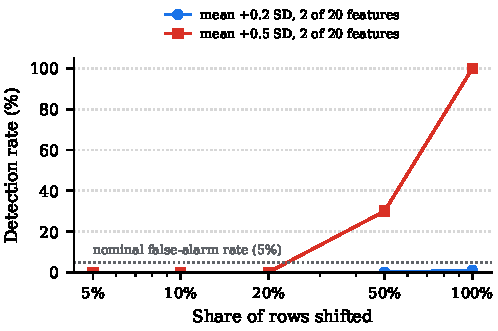
\includegraphics[width=0.92\columnwidth]{figures/fig4_calibration_power.pdf}
  \caption{Dose--response detection of a mean shift confined to a fraction of rows on a
           Gaussian pool ($d = 20$, $n = 400$, two of twenty features, $B = 199$, 200 draws
           per point; \texttt{artifacts/runs/calibrated-power-v1}). At $50\%$ of rows with
           $\delta = 0.5$ the calibrated rule declares in $30.0\%$ of draws and at full
           coverage in $100.0\%$, while a shift covering a fifth of the rows or less falls
           below the detection floor of the pathway at this sample size --- and so does the
           loose rule. The same 20\%-of-rows shift is detectable on recorded traffic, where
           the shifted rows move off a mass point rather than into a Gaussian tail
           (Table~\ref{tab:localization}); the floor is a property of the marginal, not of
           the calibration. The dotted line is the nominal false-alarm rate of 5\%; a rule
           that holds false alarms at nominal is also a rule that declines to declare when
           the evidence is not there, and this is what that costs.}
  \label{fig:calibration-power}
\end{figure}

Larger windows do not move the sparse floor. Repeating the dose--response at $n = 800$ and
$n = 1600$ (\texttt{artifacts/runs/calibrated-power-w800},
\texttt{calibrated-power-w1600}) leaves every cell at a fifth of the rows or fewer at
$0.0\%$ declared for all three statistics, up to $320$ moved rows, and the loose rule
touches only $6.0\%$ there: for a two-feature shift, a fraction of rows below a quarter of
the window is out of reach of the marginal at any window length we can afford, because the
moved mass enters the pooled distribution multiplied by that fraction. Above the floor,
window length buys power steeply --- a $+0.5\sigma$ shift on half the rows goes from
$30.0\%$ declared at $n = 400$ to $100\%$ at $n = 800$, and a $+0.2\sigma$ shift on every
row from $1.0\%$ to $95.0\%$ and then $100\%$ at $n = 1600$ --- with the calibrated rule
paying for its level exactly in the mid-range ($67.5\%$ against $95.0\%$ declared at
$n = 800$). That price is the honest cost of holding the false-alarm rate at nominal, and
it is why the sparse cells are reported as out of reach rather than tuned.
